\chapter{\label{resultados}Resultados}

Una vez finalizada la fase de desarrollo de la aplicación, en este capítulo se exponen los resultados finales obtenidos. Se detalla la solución inmersiva alcanzada mostrando las interfaces generadas, se evalúa su puesta en producción y métricas de rendimiento y se analizan los costes asociados frente a la planificación inicial. Finalmente, se realiza una reflexión académica sobre la relación del proyecto con el plan de estudios del Grado.

\section{Casos de Prueba y Modelos Arquitectónicos}
Para poner a prueba el software desarrollado, se ha probado de manera exitosa la aplicación a tres tipos de modelos arquitectónicos, demostrando una gran adaptabilidad a diferentes tipos de edificios.

\subsection{Apartamento Individual (Tres Cantos, Madrid)}
Este primer escenario representa una vivienda unifamiliar de un solo nivel. Ha sido el entorno principal empleado de forma continuada durante el ciclo de desarrollo de la aplicación, utilizándose como escena de pruebas en lugar de avanzar con los tres casos de forma simultánea. Resultó ser el modelo ideal para depurar las interacciones a corta distancia y calibrar el comportamiento de las herramientas inmersivas en espacios reducidos. Cabe destacar que, aunque el modelo de diseño teórico (BIM) comprende la vivienda en su totalidad, el acceso a la reconstrucción volumétrica de la realidad (\textit{Gaussian Splatting}) está limitado a una única habitación debido a la alta complejidad computacional y la falta de accesibilidad a dicho modelo. La proporción que tiene dicho modelo respecto a la totalidad del modelo teórico se puede apreciar en la Figura \ref{fig:trescantospiso}. 

\begin{figure}[!htb]
\centering
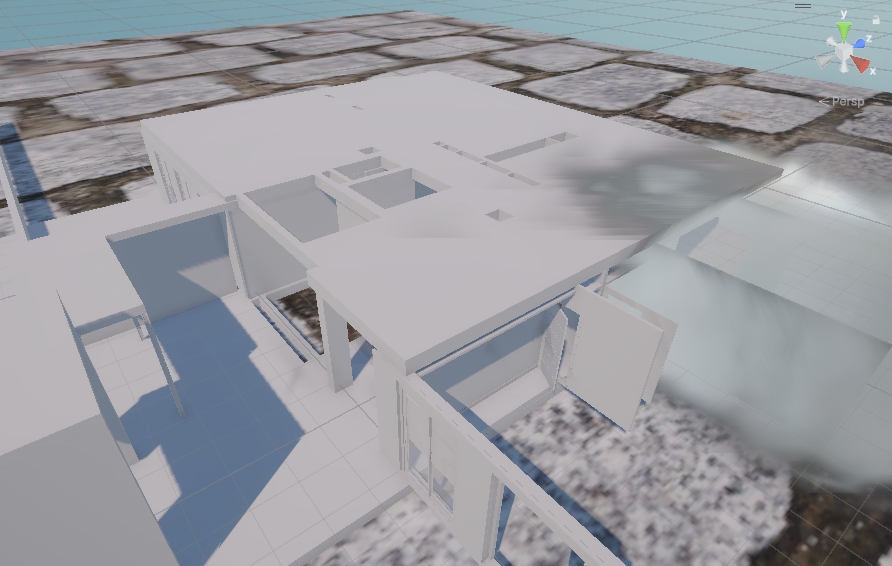
\includegraphics[width=0.8\linewidth]{include/images/trescantospiso.png}
\caption{Vista general del piso con el modelo de puntos apreciable en la parte derecha}
\label{fig:trescantospiso}
\end{figure}

\subsection{Aeródromo de la Universidad de Alicante}
Este modelo representa el entorno de la Antigua Torre de Control de las instalaciones universitarias. Al ser una estructura vertical y aislada que opera como edificio de oficinas y gestión, permitió testear los algoritmos de movimiento en desniveles (prevención de cinetosis en escaleras) y comprobar el rendimiento de los colisionadores con grandes ventanales y geometrías atípicas. Para este caso de estudio específico no se dispuso de una digitalización física de la realidad, operando exclusivamente sobre el entorno BIM para la validación de las lógicas de movimiento y físicas procedurales. En las Figuras \ref{fig:aerodromofull} y \ref{fig:aerodromo} se puede apreciar la diferencia del edificio en su totalidad con una versión descompuesta en solo puertas, ventanas, suelos y aparatos sanitarios.

\begin{figure}[!htb]
    \centering
    % ---- PRIMERA IMAGEN ----
    \begin{minipage}[b]{0.48\linewidth}
        \centering
        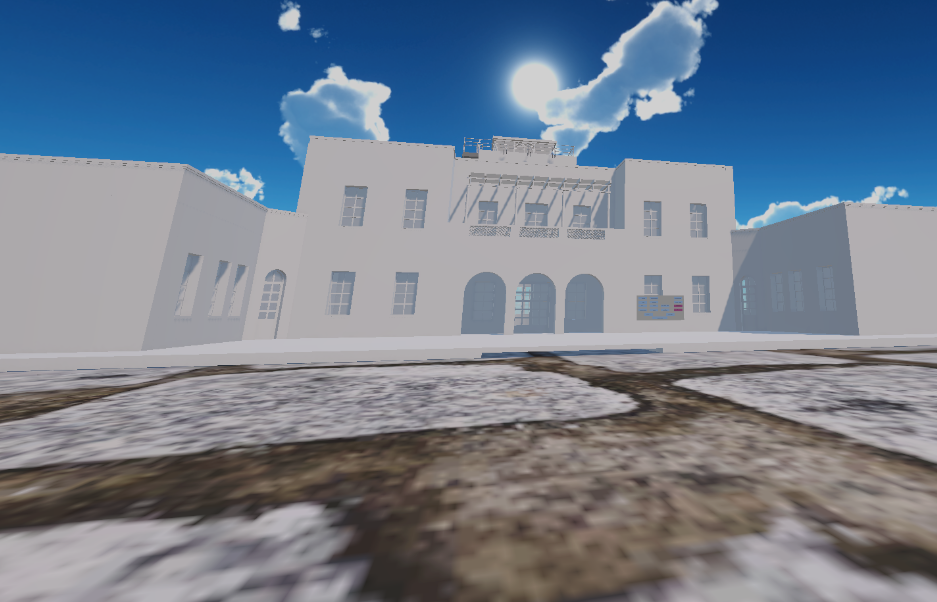
\includegraphics[width=\linewidth]{include/images/aerodromofull.png}
        \caption{Aeródromo completo en escena}
        \label{fig:aerodromofull}
    \end{minipage}
    \hfill
    % ---- SEGUNDA IMAGEN ----
    \begin{minipage}[b]{0.48\linewidth}
        \centering
        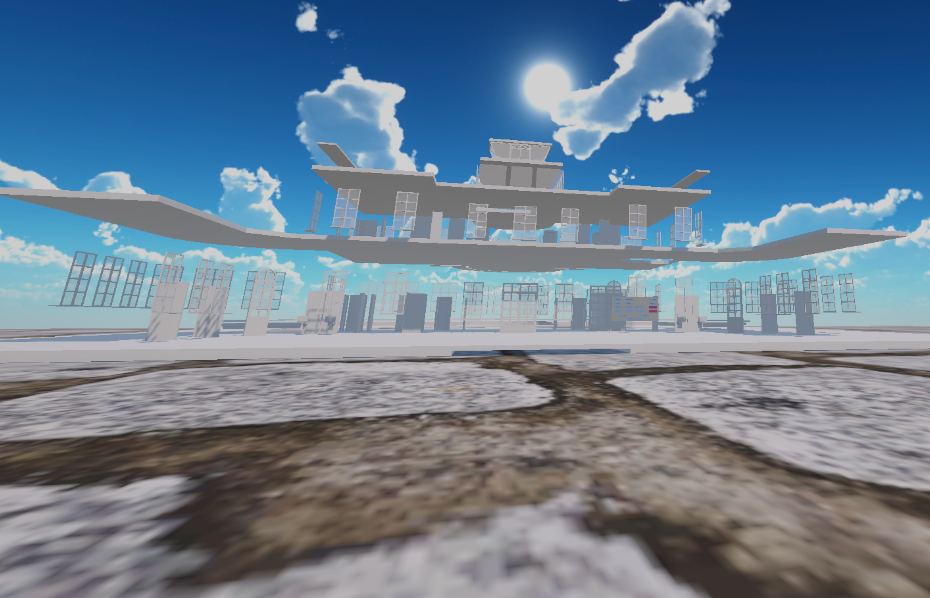
\includegraphics[width=\linewidth]{include/images/aerodromo.png}
        \caption{Aeródromo sin los muros}
        \label{fig:aerodromo}
    \end{minipage}
\end{figure}

Durante las pruebas en este modelo, se detectó que el tramo de escaleras superior tenía una pendiente excesivamente vertical, lo cual obstaculizaba el ascenso fluido del usuario mediante el sistema de movimiento continuo. Para solventar este problema de accesibilidad geométrica sin alterar la malla visual arquitectónica original, se superpuso un volumen de colisión invisible (\textit{Collider}) en forma de rampa con un ángulo de inclinación más suave. De esta forma la colisión del usuario se deslizará de manera natural hacia la planta superior, evitando bloqueos físicos o movimientos abruptos que pudieran romper la inmersión o inducir cinetosis. Visto en la Figura \ref{fig:escaleraauxiliar}.

\begin{figure}[!htb]
\centering
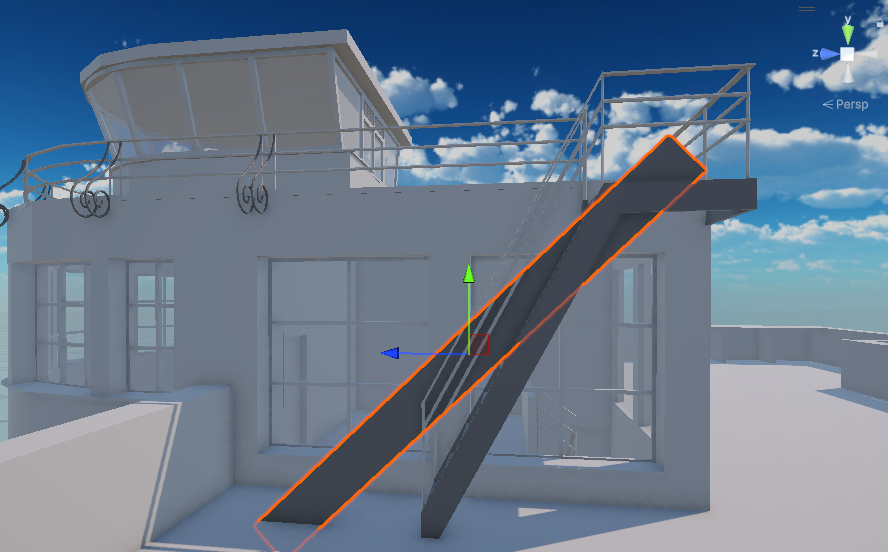
\includegraphics[width=0.8\linewidth]{include/images/escaleraauxiliar.png}
\caption{Malla de la "escalera" invisible}
\label{fig:escaleraauxiliar}
\end{figure}

\subsection{Complejo Residencial Nórdico (BIM4LCA)}
Por último, se implementó un modelo BIM altamente complejo y completo: un conjunto de apartamentos finlandés proporcionado por \textit{Nordic Sustainable Construction}. Este proyecto incluye una gran densidad poligonal y divisiones estructurales por plantas completas. Validar la aplicación en este macro-escenario sirvió como prueba para los algoritmos de optimización procedural de mallas y el gestor global de capas. 

Respecto a la representación de la obra física en este modelo, y como se anticipó en apartados anteriores de la memoria, se descartó la descarga o uso de un modelo \textit{Gaussian Splatting} de internet para evitar posibles infracciones de derechos de privacidad. Como solución técnica para probar el escáner espacial, mediante el software \textit{CloudCompare} se aisló exclusivamente la primera planta del edificio (Figura \ref{fig:thridmodel}) y se generó una nube de puntos convencional a partir del modelo teórico. Esta nube fue exportada directamente a un archivo de texto simplificado (\texttt{.txt}) para incluirlo al algoritmo de comparación de desviaciones. Como se puede observar en la Figura \ref{fig:wrongpiece}, para comprobar su funcionamiento despegó manualmente un muro del edificio.

\begin{figure}[!htb]
    \centering
    % ---- PRIMERA IMAGEN ----
    \begin{minipage}[b]{0.48\linewidth}
        \centering
        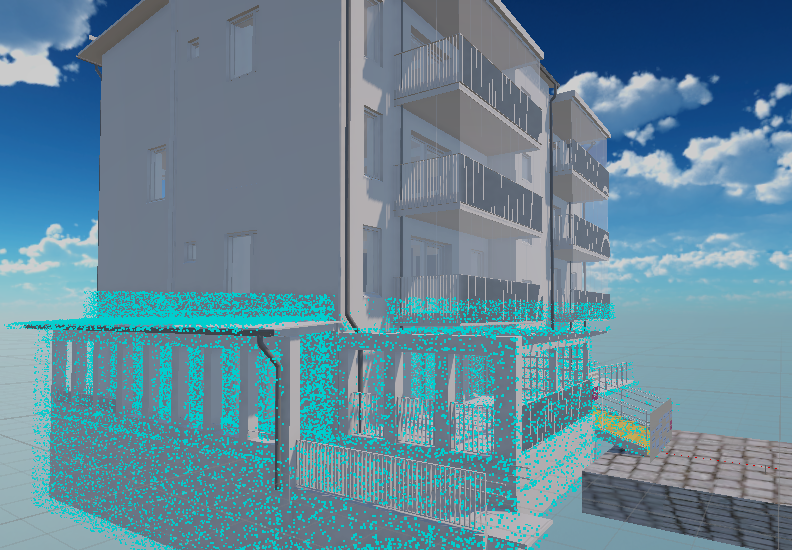
\includegraphics[width=\linewidth]{include/images/apartamentos.png}
        \caption{Edificio finlandés con modelos de puntos en el primer piso}
        \label{fig:thridmodel}
    \end{minipage}
    \hfill
    % ---- SEGUNDA IMAGEN ----
    \begin{minipage}[b]{0.48\linewidth}
        \centering
        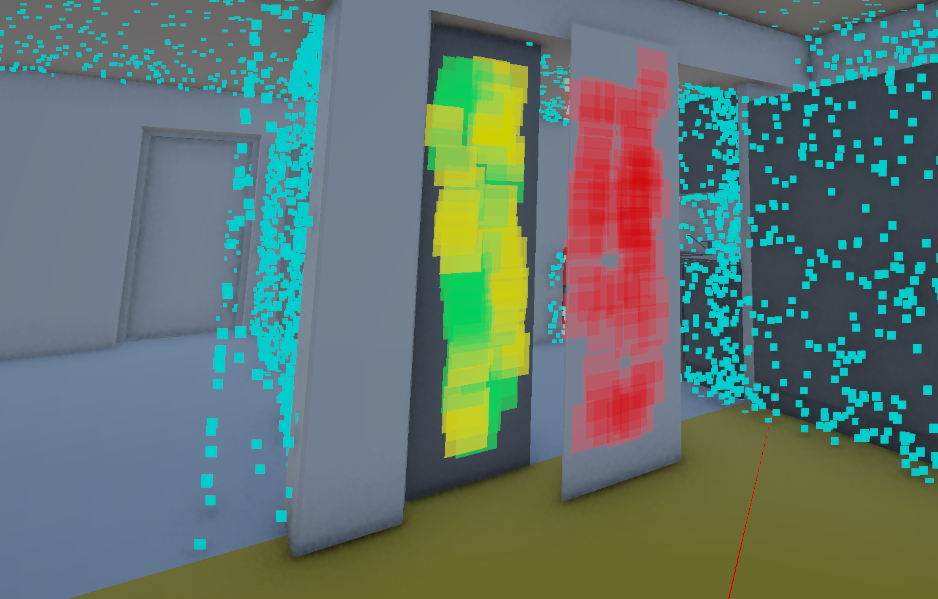
\includegraphics[width=\linewidth]{include/images/wrongpiece.png}
        \caption{Pieza desplazada marcado como rojo}
        \label{fig:wrongpiece}
    \end{minipage}
\end{figure}



\section{Descripción de la Solución Alcanzada}
El resultado principal de este proyecto es una aplicación funcional de Realidad Virtual orientada a la auditoría de obras y validación de entornos. El producto final se maneja en torno a varias interfaces y herramientas visuales operables de forma intuitiva, minimizando la carga cognitiva del operador.

\subsection{Interfaz Principal y Navegación}
Al iniciar la aplicación, el usuario accede a una sala o menú principal inmersivo. La interfaz ha sido diseñada priorizando la legibilidad espacial, previniendo el \textit{clipping} con el entorno y utilizando texturas reactivas al puntero láser. En este espacio, el operador puede consultar el registro persistente de fechas de las últimas inspecciones y seleccionar de forma fluida el entorno arquitectónico a auditar (Figura \ref{fig:res-menu}).

\begin{figure}[!htb]
\centering
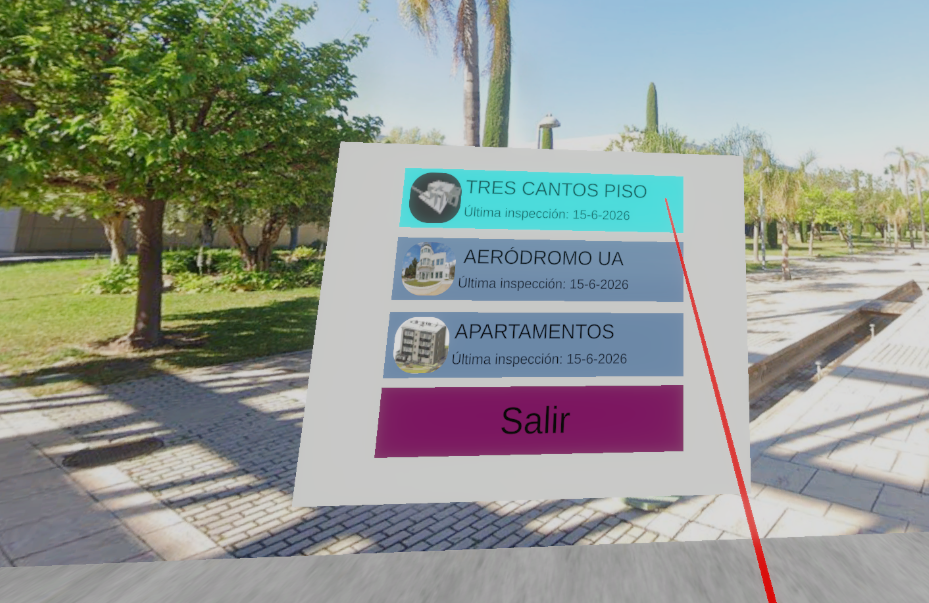
\includegraphics[width=0.8\linewidth]{include/images/figura6.1.png}
\caption{Captura del usuario en el menú principal viendo los paneles de selección de proyectos}
\label{fig:res-menu}
\end{figure}


En cada escena del edificio también se presentan botones para volver al menú principal o salir directamente de la propia aplicación.


\subsection{Herramientas de Auditoría Inmersiva}
El núcleo de la aplicación se manifiesta a través del conjunto de herramientas interactivas, las cuales devuelven resultados visuales y espaciales inmediatos al usuario:
\begin{itemize}
\item \textbf{Escáner de desviaciones (mapa de calor):} Se ha logrado proyectar visualmente la diferencia topológica entre el modelo teórico BIM y la captura de la realidad física. El resultado es un mapa de color paramétrico sobre las estructuras: verde para la coincidencia milimétrica y un degradado progresivo hacia el rojo para desviaciones estructurales críticas (Figura \ref{fig:res-escaner}).
\item \textbf{Cinta métrica y etiquetado espacial:} La herramienta genera cotas tridimensionales dinámicas que calculan distancias euclidianas exactas. Tanto estas mediciones como las etiquetas de incidencia (Graves, Leves o A Revisar) se mantienen siempre perfectamente legibles desde cualquier ángulo gracias a la técnica matemática de \textit{billboarding}.

\begin{figure}[!htb]
\centering
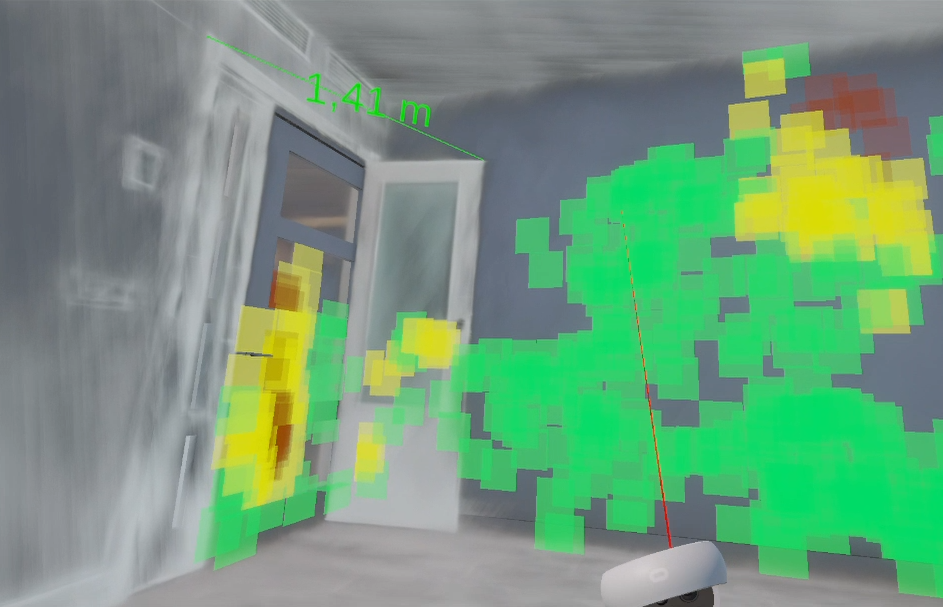
\includegraphics[width=0.8\linewidth]{include/images/figura6.2.png}
\caption{Captura desde los ojos del usuario usando el escáner de desviaciones y la cinta métrica}
\label{fig:res-escaner}
\end{figure}


\item \textbf{Gestión de capas y colisiones:} A través de un panel de control inmersivo adherido al controlador, el usuario puede aislar o deconstruir grupos estructurales masivos (Figura \ref{fig:aerodromo}). Asimismo, al ejecutar el detector de colisiones automatizado, la aplicación resalta visualmente mediante esferas las interferencias físicas entre instalaciones de conductos (MEP) y la arquitectura (Figura \ref{fig:conflicto}).
\end{itemize}

\begin{figure}[!htb]
\centering
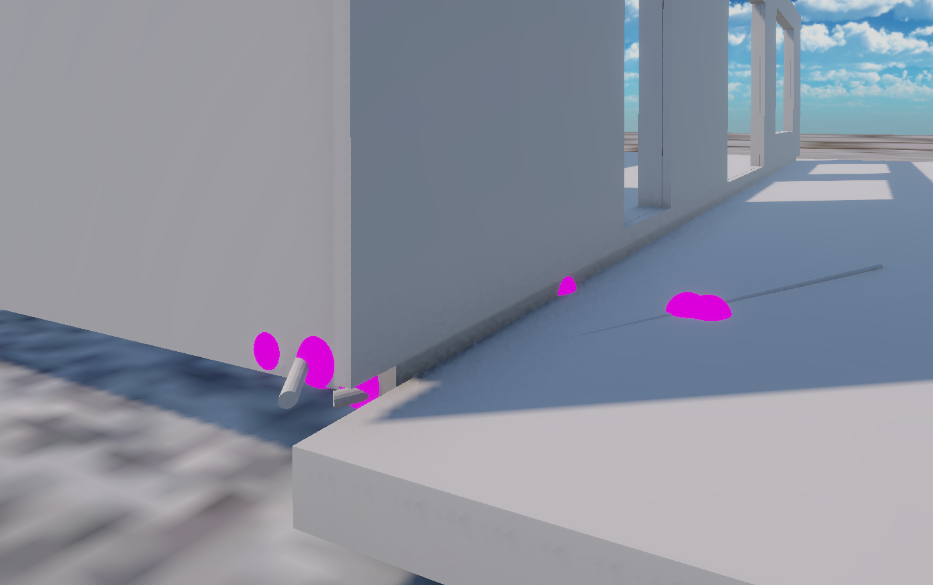
\includegraphics[width=0.8\linewidth]{include/images/conflicto.png}
\caption{Tuberías atravesando paredes y suelo en el apartamento unifamiliar}
\label{fig:conflicto}
\end{figure}


\subsection{Producto Documental: El Informe de Auditoría}
El resultado tangible y exportable del proyecto es un documento PDF generado directamente desde el entorno virtual. Tras emplear la cámara inmersiva y recopilar datos espaciales, el motor interno de maquetación compila un informe estructurado que consolida las fotografías con destellos de \textit{flash}, las incidencias categorizadas y las métricas de tolerancia de la obra. Este documento queda almacenado localmente. (Figura \ref{fig:res-pdf}).

\begin{figure}[!htb]
\centering
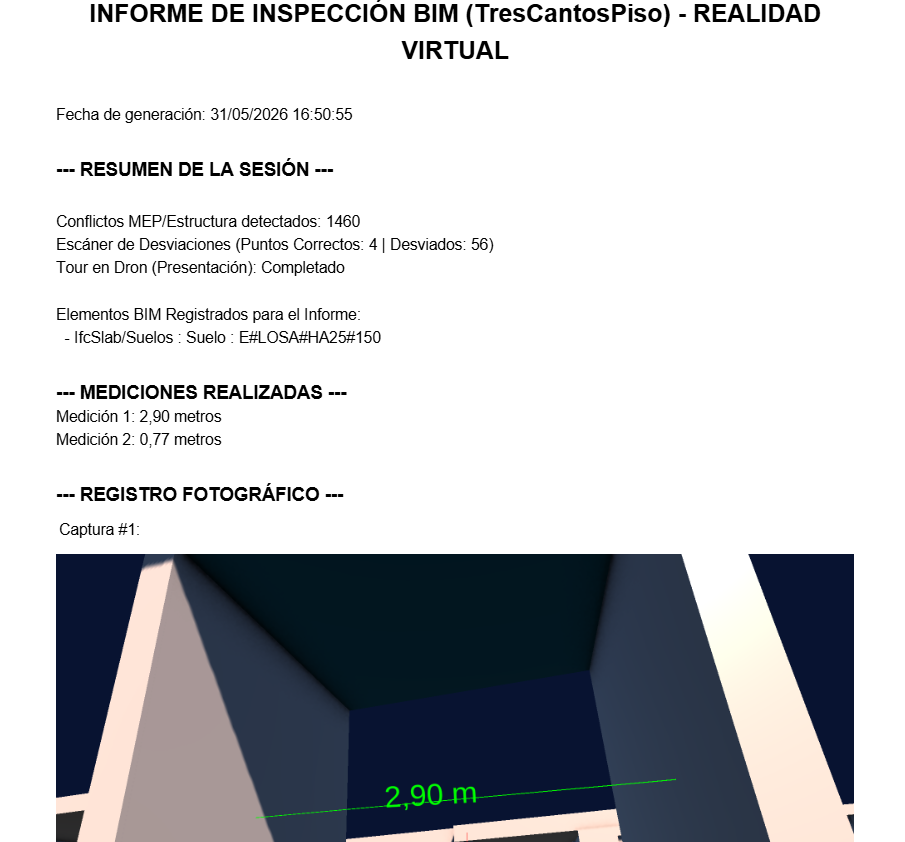
\includegraphics[width=0.8\linewidth]{include/images/figura6.3.png}
\caption{Captura de una de las páginas del PDF final generado por la aplicación (Registro fotográfico no visible)}
\label{fig:res-pdf}
\end{figure}

\section{Puesta en Producción, Métricas y Acceso}
Dada la especialización de la aplicación y el enorme peso de los modelos volumétricos, su puesta en producción excluye el despliegue masivo en tiendas de aplicaciones de consumo (\textit{App Stores}).

\begin{itemize}
\item Al trabajar con representaciones matemáticas densas como nubes de puntos pesadas y modelos BIM sin optimizar, la limitación de la memoria RAM unificada del visor (\textit{Standalone}) hace inviable la compilación en un paquete Android (\texttt{.apk}) convencional. Por ello, el modelo de despliegue recomendado consiste en generar una *Build* ejecutable nativa para entorno Windows. La aplicación se ejecuta aprovechando el cálculo de la GPU del ordenador y la experiencia visual se transmite al visor a través de cable link o por red local (\textit{Air Link}/\textit{Virtual Desktop}).
\item Al derivar la carga de procesamiento a la estación de trabajo local, la métrica de éxito más crítica, la tasa de fotogramas se mantiene alta y estable. Esto anula casi por completo la latencia visual, manteniendo la experiencia inmersiva cómoda para el usuario y minimizando el riesgo de cinetosis.
\item Las pruebas también demostraron que la arquitectura en PC permite almacenar y generar los informes PDF localmente a una velocidad superior. Además, la limpieza automática de los búferes de memoria tras la creación del documento permite ejecutar auditorías consecutivas sobre el modelo sin experimentar cierres por falta de memoria.
\end{itemize}

\section{Costes Finales y Comparativa de Planificación}
En términos de costes económicos, el desarrollo del software ha tenido un impacto financiero mínimo para la creación de este Trabajo de Fin de Grado. Se han empleado licencias académicas, repositorios gratuitos y herramientas de código abierto como el motor Unity, el procesador de nubes de puntos CloudCompare y las librerías dinámicas de C\# (iTextSharp). Los costes tangibles se limitan a la amortización técnica y energética del \textit{hardware} utilizado: el ordenador de escritorio para desarrollo y renderizado, y el visor Meta Quest 2 para el testing.

Desde el punto de vista temporal, el desarrollo se ha seguido en gran medida con la metodología de trabajo ágil (\textit{Kanban}) estipulada en las fases iniciales. Se registraron ligeras desviaciones temporales en el cronograma de investigación temprana, fundamentalmente vinculadas a incompatibilidades iniciales al renderizar el \textit{Gaussian Splatting} en Unity, así como a la adaptación a la lógica asíncrona de C\#. No obstante, estas demoras se mitigaron utilizando eficazmente los márgenes de seguridad proyectados en el cronograma, logrando desplegar un producto integral y funcional dentro del plazo académico.

\section{Viabilidad comercial}

En relación a la viabilidad comercial y vías de monetización post-académica, la aplicación desarrollada se orientaría a un modelo \textit{\gls{saas}} con suscripciones mensuales o anuales escaladas según el volumen de proyectos de la constructora.  

Los costes futuros asociados al despliegue se centrarían principalmente en el mantenimiento de la infraestructura de servidores en la nube para el almacenamiento de las nubes de puntos pesadas y el tráfico de datos de los informes. Teniendo en cuenta que el coste de reparar un fallo estructural menor detectado de forma tardía en una obra real suele superar con creces el precio de una licencia de software anual, el retorno de la inversión (ROI) para las empresas del sector resulta competitivo, consolidando la viabilidad comercial a largo plazo de esta solución tecnológica.

















\subsection{Experimento FPS vs Puntos}

Para medir el límite computacional de la aplicación durante su ejecución, se realizaron mediciones de FPS a la escena principal como prueba. Consistió en evaluar la tasa de fotogramas ante distintas cargas de densidad del modelo \textit{Gaussian Splatting}, aplicando simplificaciones sobre ésta (842.344 puntos). 

Los resultados de las cuatro pruebas realizadas se detallan en el Cuadro~\ref{tab:fps_splatting}:

\begin{table}[!htb]
    \centering
    \caption{Rendimiento de la aplicación según la densidad volumétrica (\textit{Gaussian Splatting})}
    \label{tab:fps_splatting}
    \begin{tabular}{lccc}
        \toprule
        \textbf{Categoría / Calidad} & \textbf{Porcentaje} & \textbf{Nº de Puntos} & \textbf{Tasa media (FPS)} \\
        \midrule
        Calidad Original (Nivel 1) & 100\,\% & 842.344 & 15 \\
        Simplificación Leve (Nivel 2) & 75\,\% & 631.758 & 18 \\
        Simplificación Media (Nivel 3) & 50\,\% & 421.172 & 18 \\
        Simplificación Alta (Nivel 4) & 25\,\% & 210.586 & 23 \\
        \bottomrule
    \end{tabular}
\end{table}

El análisis de los datos del experimento permite extraer dos conclusiones fundamentales sobre la arquitectura del sistema:

\begin{enumerate}
    \item \textbf{Estancamiento del rendimiento:} Al reducir la cantidad de puntos un 25\,\% (Nivel 2), el visor experimenta una leve mejora de 3 FPS. Sin embargo, al simplificar la muestra hasta la mitad exacta (Nivel 3), se mantiene estancado en los mismos 18 FPS. Este comportamiento demuestra que, una vez reducido el número de puntos, el problema ya no es la cantidad de datos, sino el esfuerzo que debe realizar la tarjeta gráfica para dibujar y superponer los elementos semitransparentes en la pantalla.
    \item \textbf{Inviabilidad autónoma (.apk):} Incluso aplicando una simplificación extrema que elimina tres cuartas partes del modelo (Nivel 4), el hardware del ordenador apenas logra alcanzar los 23 FPS, situándose muy por debajo del umbral mínimo de los 72 FPS exigidos por la industria para prevenir la cinetosis en Realidad Virtual.
\end{enumerate}

Estas mediciones apoyan la decisión de que la ejecución de digitalizaciones complejas mediante \textit{Gaussian Splatting} en visores requiere de forma obligatoria derivar la carga gráfica a un ordenador externo mediante transmisión.




































\section{Vinculación Académica sobre el Grado}
El diseño de este proyecto representa la culminación práctica de múltiples competencias, lógicas y metodologías asimiladas a lo largo de la titulación en Ingeniería Multimedia. El producto final de esta aplicación es resultado de aplicar conocimientos provenientes de las siguientes áreas:

\begin{itemize}
\item \textbf{Realidad Virtual (21040):} Durante este curso 2025-2026 en el grado se ha impartido esta asignatura, y ha sido una de las más relacionadas con el trabajo, otorgando experiencia similar en un motor diferente, Unreal Engine. Se han puesto en práctica fundamentos tales como el trazado de rayos (\textit{Raycasting}), interacción de 6DoF con mandos, y la prevención de la cinetosis a través de la interfaz.
\item \textbf{Usabilidad y Accesibilidad (21013):} Las directrices de estas materias han sido imprescindibles para el diseño de paneles de interfaces de usuario inmersivas, traduciendo elementos convencionales 2D (\textit{Canvas}) a espacios euclidianos interactivos. Se priorizó el contraste en los menús y la accesibilidad para usuarios que pudiesen padecer fatiga ocular en inmersiones prolongadas.
\item \textbf{Estructura de Datos y Algoritmia (21014):} Ha sido fundamental para la lógica del código; empleando diccionarios, *HashSets* paramétricos, listas dinámicas y árboles para aislar y procesar de manera concurrente los miles de componentes y metadatos que conforman la topología BIM.
\item \textbf{Fundamentos de videojuegos (21027) y Análisis y Especificación de Sistemas Multimedia (21017):} Proveyeron la base del flujo de trabajo: adopción de ciclos de trabajo de la metodología ágil, el diseño del modelo documental de arquitectura de software, el dominio de los repositorios de control de versiones (Git) y la correcta especificación funcional ante requerimientos cambiantes y desafíos técnicos inesperados.
\item \textbf{Dispositivos e Infraestructuras para Sistemas Multimedia (21021):} Respecto a la parte teórica contribuyó a la investigación del estado del arte, proporcionando información sobre los distintos tipos de pantalla (por ejemplo LCD), procesadores integrados en el propio equipo informático (SoC), o conceptos como IoT.
\item \textbf{Administración de empresas (21004):} Ha resultado útil para la elaboración del estudio de viabilidad, demostrando que, previo a cualquier desarrollo técnico, llega a ser prácticamente crucial realizar un estudio de mercado. La elaboración del modelo \textit{Lean Canvas}, hecho durante la materia ha permitido analizar de forma estructurada la viabilidad comercial de llevar a cabo este proyecto.
\end{itemize}